\documentclass[a4paper,10pt]{report}\input{../0.Préambule/Préambule_cours_prof}\input{0_Préambule_Proba}\begin{document}

\newpage
\setcounter{chapter}{15}
\hypertarget{Probabilites}{}
\chapter{Probabilités}

\paragraph*{Objectif du chapitre :}
\begin{enumerate}
\item[•] Connaître et utiliser le vocabulaire univers, expérience aléatoire, événement, éventualité et issues.
\item[•] Comprendre et interpréter un événement contraire, une intersection ou réunion d'événements.
\item[•] Reconnaître et utiliser une situation d'équiprobabilité.
\item[•] Calculer des probabilités à l'aide d'une distribution de fréquences, d'un arbre des possibles ou d'un tableau.
\end{enumerate}

\section{Vocabulaire des événements} 

\begin{dft}
   Chaque résultat possible et prévisible d'une expérience aléatoire est appelé \textbf{éventualité}.
\end{dft}

\begin{ex}
   \begin{enumerate}
      \item[•] Lancer un dé à six faces : \og obtenir un $2$ \fg{} est une éventualité de cette expérience aléatoire,
      \item[•] Tirage des six numéros gagnants du Loto : \og obtenir la combinaison \og{} $2-5-17-23-36-41$ \fg{} est une éventualité de cette expérience aléatoire.
   \end{enumerate}
\end{ex}

\begin{dft}
   L'ensemble formé par les éventualités est appelé \textbf{univers}, il est très souvent noté $\Omega$.
\end{dft}

\begin{ex}
   \begin{enumerate}
      \item[•] Lancer d'une pièce de monnaie : $\Omega =\{$~pile~;~face~$\}$,
      \item[•] lancer un dé à six faces : $\Omega =\{~1~;~2~;~3~;~4~;~5~;~6~\}$.
   \end{enumerate}
\end{ex}

\begin{dft}
   \begin{enumerate}
      \item[•] Un \textbf{événement} de l'expérience aléatoire est une partie quelconque de l'univers,
      \item[•] Un événement ne comprenant qu'une seule éventualité est un \textbf{événement élémentaire}.
   \end{enumerate}
\end{dft}

\begin{ex}
   \begin{enumerate}
      \item[•] $A=$ \og obtenir un $5$ \fg{} est un événement élémentaire que l'on peut noter $A=\{~5~\}$,
      \item[•] $B=$ \og obtenir un numéro pair \fg{} est un événement que l'on peut noter $B=\{~2~;~4~;~6~\}$.
   \end{enumerate}
\end{ex}

\begin{dft}
   \begin{enumerate}
      \item[•] L'événement qui ne contient aucune éventualité est l'\textbf{événement impossible}, noté $\varnothing$,
      \item[•] l'événement composé de toutes les éventualités est appelé \textbf{événement certain}.
   \end{enumerate}
\end{dft}

\begin{ex}
   \begin{enumerate}
      \item[•] Tirage des six numéros gagnants du loto : \og obtenir la combinaison $3-25-38-59-67-91$ \fg{} est un événement impossible (les numéros vont de $1$ à $49$),
      \item[•] Lancer d'un dé à six faces : \og obtenir un nombre positif \fg{} est un événement certain.
   \end{enumerate}
\end{ex}

\begin{dft}
   Pour tout événement $A$ il existe un événement noté $\overline{A}$ et appelé \textbf{événement contraire} (ou complémentaire) de $A$, qui est composé des éléments de $\Omega$ qui ne sont pas dans A.
\end{dft}

\begin{ex}
   \begin{enumerate}
      \item[•] Lancer d'une pièce de monnaie : si $A=\{\text{~pile~}\}$ alors son événement contraire est $\overline{A}=\{\text{~face~}\}$,
      \item[•] Lancer d'un dé à six faces : si $A$ est l'événement \og obtenir un nombre inférieur ou égal à $4$ \fg{}, alors son événement contraire $\overline{A}$ est l'événement \og obtenir $5$ ou $6$ \fg{}.
   \end{enumerate}
\end{ex}

\section{Intersection et réunion d'événements}

\begin{dft}
Soit $A$ et $B$ deux événements de $\Omega$.

\vspace{-5mm}
\begin{minipage}{9cm}
\textbf{Intersection d'événements} : l'événement constitué des éventualités appartenant à $A$ et à $B$ est noté $A\cap B$ \\(se lit \og $A$ inter $B$ \fg{} ou \og $A$ et $B$ \fg)
\end{minipage}
\begin{minipage}{5cm}
\begin{center}
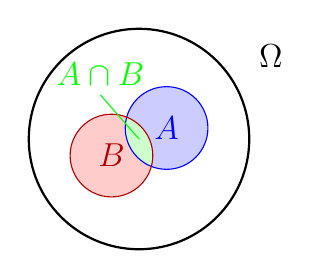
\begin{tikzpicture}[scale=0.7]
\draw[color=black,thick] (0,0) circle (2cm);
\node[color=black,right] at (2cm,1.5cm) {\large{$\Omega$}};
\fill[fill=blue!20] (0.5cm,0.2cm) circle (0.75cm);
\fill[fill=red!20] (-0.5cm,-0.3cm) circle (0.75cm);
\begin{scope}
\clip (0.5cm,0.2cm) circle (0.75cm);
\fill[fill=green!20] (-0.5cm,-0.3cm) circle (0.75cm);
\end{scope}
\draw[color=blue] (0.5cm,0.2cm) circle (0.75cm) node {\large{$A$}};
\draw[color=red!70!black] (-0.5cm,-0.3cm) circle (0.75cm) node {\large{$B$}};
\draw[color=green] (0,0)--(-0.7cm,0.8cm) node[above] {\large{$A\cap B$}};
%\fill[fill=violet!20] (2.125cm,-1.5cm) rectangle +(0.5cm,0.5cm) node[color=violet,pos=0.5,right=0.25cm] {$P$};
\end{tikzpicture}
\end{center}
\end{minipage}

\vspace{-5mm}
\begin{minipage}{5cm}
\begin{center}
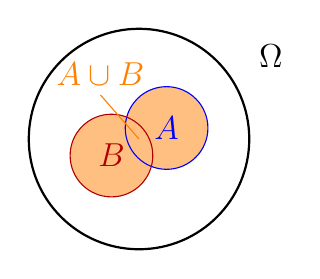
\begin{tikzpicture}[scale=0.7]
\draw[color=black,thick] (0,0) circle (2cm);
\node[color=black,right] at (2cm,1.5cm) {\large{$\Omega$}};
\fill[fill=orange!50] (0.5cm,0.2cm) circle (0.75cm);
\fill[fill=orange!50] (-0.5cm,-0.3cm) circle (0.75cm);
\begin{scope}
\clip (0.5cm,0.2cm) circle (0.75cm);
\fill[fill=orange!50] (-0.5cm,-0.3cm) circle (0.75cm);
\end{scope}
\draw[color=blue] (0.5cm,0.2cm) circle (0.75cm) node {\large{$A$}};
\draw[color=red!70!black] (-0.5cm,-0.3cm) circle (0.75cm) node {\large{$B$}};
\draw[color=orange] (0,0)--(-0.7cm,0.8cm) node[above] {\large{$A\cup B$}};
%\fill[fill=violet!20] (2.125cm,-1.5cm) rectangle +(0.5cm,0.5cm) node[color=violet,pos=0.5,right=0.25cm] {\large{$P$}};
\end{tikzpicture}
\end{center}
\end{minipage}
\begin{minipage}{9.5cm}
\textbf{Réunion d'événements} : l'événement constitué des éventualités appartenant à $A$ ou à $B$ est noté $A\cup B$ \\(se lit $A$ et de $B$ ou \og $A$ union $B$ \fg{} ou \og $A$ ou $B$ \fg).
\end{minipage}
\end{dft}

\begin{rmq}
   Si $A\cap B=\varnothing$, on dit que les événements sont \textbf{disjoints} ou \textbf{incompatibles}.
\end{rmq}

\begin{ex}
   On considère un jeu de $52$ cartes. On note $A$ l'événement \og obtenir une carte paire \fg{} et $B$ l'événement \og obtenir une carte de valeur inférieure strictement à six \fg.
  \begin{enumerate}
  \item[] $A\cap B=$ \og obtenir une carte paire et inférieures strictement à six \fg{} : $A \cap B=\{~2~;~4~\}$,
  \item[] $A \cup B=$ \og obtenir une carte paire ou inférieure strictement à six \fg{} : $A \cup B=\{~1~;~2~;~3~;~4~;~5~;~6~;~8~;~10~\}$.
  \end{enumerate}
\end{ex}

\section{Calcul de probabilités} 

\begin{dft}
   La \textbf{probabilité} d'un événement est la somme des probabilités des événements élémentaires qui le constituent.
\end{dft}  

\begin{ex}
On lance un dé non pipé à six faces. La probabilité d'obtenir un nombre pair est égale à la probabilité d'obtenir un 2 plus la probabilité d'obtenir un 4 plus la probabilité d'obtenir un 6:
\[P({2;4;6})=P({2})+P({4})+P({6})\]
\end{ex}

\begin{dft}
On dit qu'il y a \textbf{équiprobabilité} lorsque tous les événements élémentaires ont la même probabilité,
\end{dft}  

\begin{rmq}
  Dans un exercice, pour signifier qu'on est dans une situation d'équiprobabilité on a généralement dans l'énoncé un expression du type :
  \begin{enumerate}
     \item[•] on lance un dé \textbf{non pipé},
     \item[•] dans une urne, il y a des boules \textbf{indiscernables} au toucher,
     \item[•] on rencontre au \textbf{hasard} une personne parmi \dots
  \end{enumerate}
\end{rmq}

\begin{prop}
Dans une situation d'équiprobabilité, on a : $P(A) =\dfrac{\textrm{nombre d'éléments de }A}{\textrm{nombre d'éléments de }\Omega} =\dfrac{\textrm{Card}(A)}{\textrm{Card}(\Omega)}$.
\end{prop}

\begin{ex}
  On lance un dé équilibré à six faces. \\
  On considère les événements $A$ : \og obtenir un chiffre pair \fg{} et l'événement $B$ : \og obtenir un diviseur de six \fg{}.
   \begin{enumerate}
      \item[] Le dé est équilibré donc on est dans une situation d'équiprobabilité,
      \item[] $A=\{~2~;~4~;~6~\}$ \quad donc, $P(A)=\dfrac{\textrm{nombre d'éléments de }A}{\textrm{nombre d'éléments de }\Omega} =\dfrac{3}{6}=\dfrac{1}{2}$
      \item[] $B=\{~1~;~2~;~3~;~6~\}$ \quad donc, $P(B)=\dfrac{\textrm{nombre d'éléments de }B}{\textrm{nombre d'éléments de }\Omega} =\dfrac{4}{6}=\dfrac{2}{3}$.
   \end{enumerate}
\end{ex}

\begin{prop}
Soit $A$ et $B$ deux événements, on a les propriétés suivantes :

\begin{minipage}{8cm}
\begin{enumerate}
\item[•] $P(\varnothing)=0$
\item[•] $P(\Omega)=1$
\end{enumerate}
\end{minipage}
\begin{minipage}{9cm}
\begin{enumerate}
\item[•] $0 \leqslant P(A) \leqslant 1$
\item[•] $P(\overline{A})=1-P(A)$
\item[•] $P(A\cup B)=P(A)+P(B)-P(A\cap B)$
\end{enumerate}
\end{minipage}
\end{prop}

\begin{ex}
On considère l'ensemble $E$ des entiers de $1$ à $20$. On choisit l'un de ces nombres au hasard. \\
$A$ est l'événement : \og le nombre est multiple de $3$ \fg{} et $B$ est l'événement : \og le nombre est multiple de $2$ \fg.
   
\begin{minipage}{7cm}
\begin{enumerate}
\item[] $P(A)=\dfrac{6}{20}=\dfrac{3}{10}=0,3$.
\item[] $P(\overline{A})=1-P(A)=1-\dfrac{3}{10}=\dfrac{7}{10}=0,7$.
\item[] $P(B)=\dfrac{10}{20}=\dfrac{1}{2}=0,5$.
\end{enumerate}
\end{minipage}
\begin{minipage}{9cm}
\begin{enumerate} 
\item[] $P(A \cap B)=\dfrac{3}{20}=0,15$.
\item[] $P(A \cup B)=p(A)+p(B)-p(A\cap B)=\dfrac{6}{20}+\dfrac{10}{20}-\dfrac{3}{20}=\dfrac{13}{20}$.
\end{enumerate}
\end{minipage}
\end{ex}

\section{Représentation des événements} 

\noindent \begin{minipage}{8.5cm}
\textbf{Diagramme de Venn ou \og patates \fg }

Représentation graphique de l'intersection et de la réunion d'événements :

Soit A et B deux parties (ou sous populations) d'une population E.

\begin{center}
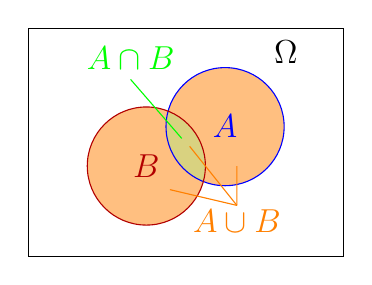
\begin{tikzpicture}
\filldraw[fill=white] (-2,-1.45) rectangle (2,1.45);
\node[color=black,right] at (1cm,1.15cm) {\large{$\Omega$}};
\fill[fill=orange!50] (0.5cm,0.2cm) circle (0.75cm);
\fill[fill=orange!50] (-0.5cm,-0.3cm) circle (0.75cm);
\begin{scope}
\clip (0.5cm,0.2cm) circle (0.75cm);
\fill[fill=green!30!orange!50] (-0.5cm,-0.3cm) circle (0.75cm);
\end{scope}
\draw[color=blue] (0.5cm,0.2cm) circle (0.75cm) node {\large{$A$}};
\draw[color=red!70!black] (-0.5cm,-0.3cm) circle (0.75cm) node {\large{$B$}};
\draw[color=green] (-0.05,0.05)--(-0.7cm,0.8cm) node[above] {\large{$A\cap B$}};
\draw[color=orange] (0.05,-0.05)--(0.65cm,-0.8cm);
\draw[color=orange] (-0.2,-0.6)--(0.65cm,-0.8cm);
\draw[color=orange] (0.65,-0.3)--(0.65cm,-0.8cm);
\node[color=orange] at (0.65cm,-1cm) {\large{$A\cup B$}};
%\fill[fill=violet!20] (2.125cm,-1.5cm) rectangle +(0.5cm,0.5cm) node[color=violet,pos=0.5,right=0.25cm] {$P$};
\end{tikzpicture}
\end{center}
\end{minipage}
\hspace{5mm}
\begin{minipage}{7.5cm}
\textbf{Tableaux}

On jette deux dés à quatre faces (tétraèdre régulier) et on calcule le produit obtenu :

\begin{center}
   \renewcommand{\arraystretch}{1.65}
   \begin{tabular}{|*{5}{C{0.5}|}}
      \hline 
      & \textbf{1} & \textbf{2} & \textbf{3} & \textbf{4} \\ 
      \hline
      \textbf{1} & $1$ & $2$ & $3$ & $4$ \\ 
      \hline
      \textbf{2} & $2$ & $4$ & $6$ & $8$ \\ 
      \hline 
      \textbf{3} & $3$ & $6$ & $9$ & $12$ \\ 
      \hline 
      \textbf{4} & $4$& $8$ & $12$ & $16$ \\ 
      \hline 
   \end{tabular} 
\end{center}
\end{minipage}

\noindent \textbf{Arbres}

On lance une pièce de monnaie trois fois de suite, on peut schématiser cette expérience par un arbre :

\begin{center}
% Racine à Gauche, développement vers la droite
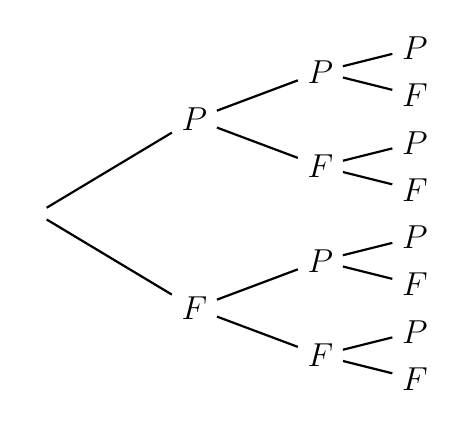
\begin{tikzpicture}[xscale=1,yscale=1,scale=0.6]
% Styles (MODIFIABLES)
\tikzstyle{fleche}=[-,>=latex,thick]
\tikzstyle{noeud}=[fill=white]
\tikzstyle{feuille}=[fill=white]
\tikzstyle{etiquette}=[midway,above]
\tikzstyle{etiquette1}=[midway,below]
% Dimensions (MODIFIABLES)
\def\DistanceInterNiveaux{2}
\def\DistanceInterFeuilles{1}
% Dimensions calculées (NON MODIFIABLES)
\def\NiveauA{(0)*\DistanceInterNiveaux}
\def\NiveauB{(1.6666666666666665)*\DistanceInterNiveaux}
\def\NiveauC{(3)*\DistanceInterNiveaux}
\def\NiveauD{(4)*\DistanceInterNiveaux}
\def\InterFeuilles{(-1)*\DistanceInterFeuilles}
% Noeuds (MODIFIABLES : Styles et Coefficients d'InterFeuilles)
\node[noeud] (R) at ({\NiveauA},{(3.5)*\InterFeuilles}) {};
\node[noeud] (Ra) at ({\NiveauB},{(1.5)*\InterFeuilles}) {\large{$P$}};
\node[noeud] (Raa) at ({\NiveauC},{(0.5)*\InterFeuilles}) {\large{$P$}};
\node[feuille] (Raaa) at ({\NiveauD},{(0)*\InterFeuilles}) {\large{$P$}};
\node[feuille] (Raab) at ({\NiveauD},{(1)*\InterFeuilles}) {\large{$F$}};
\node[noeud] (Rab) at ({\NiveauC},{(2.5)*\InterFeuilles}) {\large{$F$}};
\node[feuille] (Raba) at ({\NiveauD},{(2)*\InterFeuilles}) {\large{$P$}};
\node[feuille] (Rabb) at ({\NiveauD},{(3)*\InterFeuilles}) {\large{$F$}};
\node[noeud] (Rb) at ({\NiveauB},{(5.5)*\InterFeuilles}) {\large{$F$}};
\node[noeud] (Rba) at ({\NiveauC},{(4.5)*\InterFeuilles}) {\large{$P$}};
\node[feuille] (Rbaa) at ({\NiveauD},{(4)*\InterFeuilles}) {\large{$P$}};
\node[feuille] (Rbab) at ({\NiveauD},{(5)*\InterFeuilles}) {\large{$F$}};
\node[noeud] (Rbb) at ({\NiveauC},{(6.5)*\InterFeuilles}) {\large{$F$}};
\node[feuille] (Rbba) at ({\NiveauD},{(6)*\InterFeuilles}) {\large{$P$}};
\node[feuille] (Rbbb) at ({\NiveauD},{(7)*\InterFeuilles}) {\large{$F$}};
% Arcs (MODIFIABLES : Styles)
\draw[fleche] (R)--(Ra);
\draw[fleche] (Ra)--(Raa);
\draw[fleche] (Raa)--(Raaa);
\draw[fleche] (Raa)--(Raab);
\draw[fleche] (Ra)--(Rab);
\draw[fleche] (Rab)--(Raba);
\draw[fleche] (Rab)--(Rabb);
\draw[fleche] (R)--(Rb);
\draw[fleche] (Rb)--(Rba);
\draw[fleche] (Rba)--(Rbaa);
\draw[fleche] (Rba)--(Rbab);
\draw[fleche] (Rb)--(Rbb);
\draw[fleche] (Rbb)--(Rbba);
\draw[fleche] (Rbb)--(Rbbb);
\end{tikzpicture}
\end{center}

\end{document}